%%
%% Dit is een subdocument van het projectplan.
%%

\subsection{Introductie}
Het project betreft het herbouwen van het WickedXmas tool, omdat de tool gebruikt wordt voor studie
en ontwerp van chips is het belangrijk dat deze tool foutloos werkt. Verder betreft het een niet
alledaags domein waardoor er extra aandacht noodzakelijk is om het domein te verkennen. De eis dat
het tool platformonafhankelijk moet zijn en bij voorkeur in C++ geschreven is , maken dat er tijd
voorzien moet worden om de teamleden de nodige ontwikkeltools eigen te maken.
Er is gekozen voor agile aanpak zoals in DAD, het plan is opgebouwd volgens de
drie fasen ervan.

\subsection{Organisatie}
 De teamleden ontwikkelen gedelokaliseerd en communiceren via internet. Sources worden gecentraliseerd
 in de cloud met versiebeheer. Het team beschikt over een begeleider welke toeziet op de gang van zaken
 en geeft op vraag advies. De opdrachtgever en tevens domeinspecialist kan geraadpleegd worden voor
 specifieke domein vragen en evaluatie van het product.
 \begin{enumerate}
 	\item Guus Bonnema
 	\begin{itemize}
		\item Rol - Ontwikkelaar
		\item Skills - IT, Java, Linux
	\end{itemize}
 	\item Jeroen Kleijn
 	\begin{itemize}
		\item Rol - Ontwikkelaar
		\item Skills - IT , MS VisualStudio (C\#), C/C++, Java, Linux + Windows
	\end{itemize}
 	\item Stefan Versluys
 	\begin{itemize}
		\item Rol - Ontwikkelaar
		\item Skills - IT , MS VisualStudio (C\#), C/C++, Java, Windows + VxWorks
	\end{itemize}
	\item Freek Verbeek
	\begin{itemize}
		\item Rol - Proces begeleider
	\end{itemize}
	\item Bernard van Gastel
	\begin{itemize}
		\item Rol - Opdrachtgever / Domeinspecialist : begeleid inhoudelijk
	\end{itemize}

 \end{enumerate}

\subsection{Hardware en software}
\begin{enumerate}
	\item Voor versiebeheer en sources te borgen wordt een centrale Git repo gebruikt.
	\item Communicatie middelen zijn GitHub, gmail, skype , teamviewer.
	\item Platformonafhankelijke IDE met C++ compiler.
	\item Platformonafhankelijke GUI Toolkit.
	\item Componenten voor xmas analyse en checks.
	\item Mac OS , MS Windows, Linux platformen.
	\item DAD Support Tool (Work Item template)
\end{enumerate}


\subsection{DAD Ontwikkelmethode}
\subsubsection{Lifecycle}

\begin{figure}[h]
  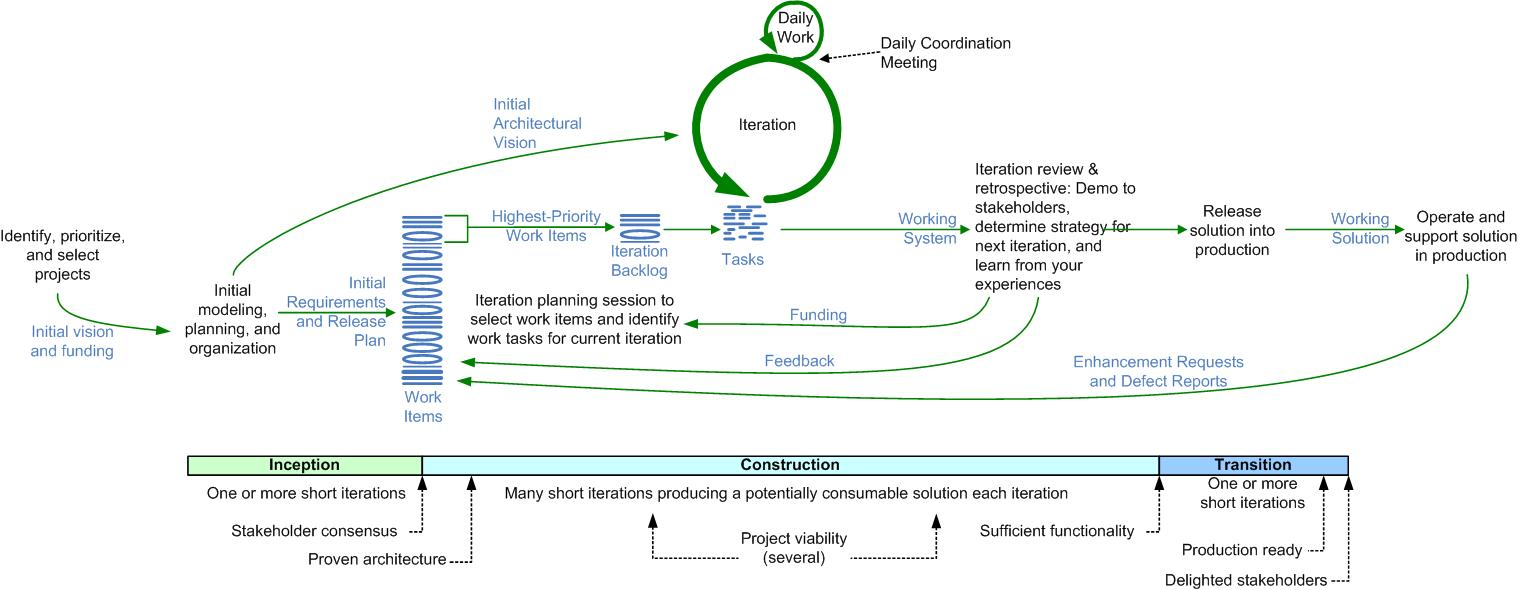
\includegraphics[width=1.0\textwidth]{dadLifecycleUP2}
  \caption{DAD basic Lifecycle} 
\end{figure}
Mijlpalen : 
\begin{enumerate}
\item Stakeholder consensus
\item Proven architecture
\item Sufficient functionality
\item Production ready
\item Delighted stakeholders
\end{enumerate}

\subsubsection{Iteratie aanpak}
\begin{itemize}
 \item Analyse : Modellen, requirements , prioriteiten en selectie 
 \item (Test Driven) Development
 \item Refactoring
 \item Peer review
 \item Levert steeds iets bruikbaars op dat ge\"evalueerd kan worden voor feedback.
 \item Planning
 \item Documentatie ( ,scriptie, onderzoekscontext) 
\end{itemize}



